\section{Adversarial Search}
\subsection{Minimax}
Maximize your minimum gain. Assume opponent plays optimally.
\subsubsection{Alpha-Beta Pruning}
\begin{figure}[H]
\centering
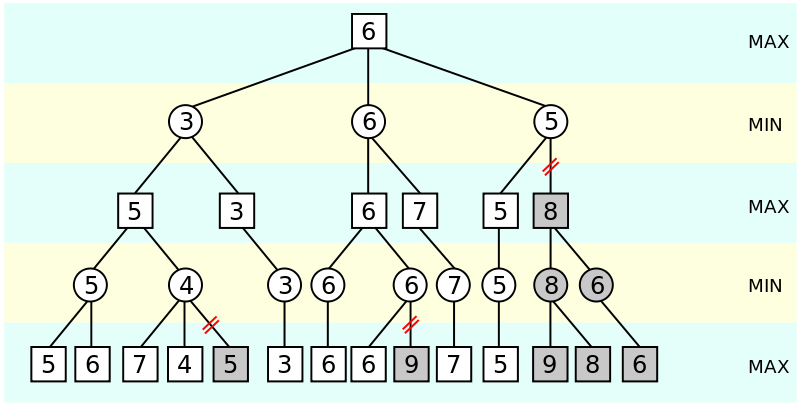
\includegraphics[width=\linewidth]{alpha-beta-pruning}
\end{figure}

Idea: If we are at a max-node, and we found the value $v$ of a child. The value of the max-node must be $\geq v$. 
Leverage this information when searching the other children.

\subsection{Expectimax}
Minimize the expected value of your opponents actions. Assume opponents play randomly instead of optimally. Can prune if we have bounds on the utility of terminal states. With this info, we can compute upper and lower bounds on the expected value of a chance node.